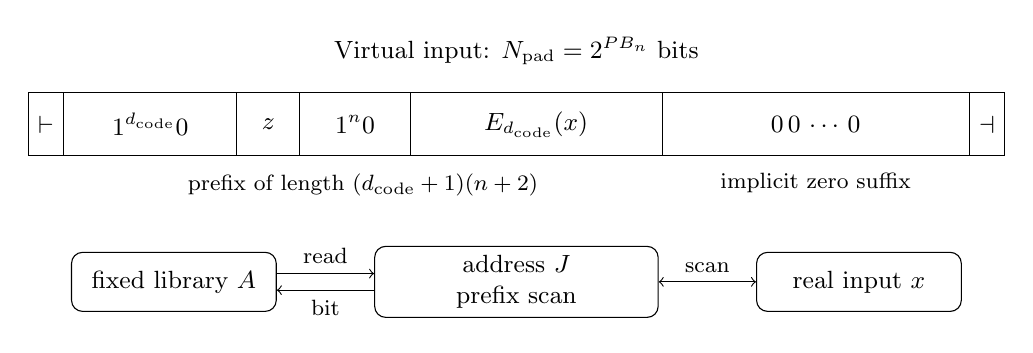
\begin{tikzpicture}[x=1cm,y=1cm,font=\small]
  \draw (0,0) rectangle (12.4,0.8);
  \draw (0.45,0) -- (0.45,0.8);
  \draw (2.65,0) -- (2.65,0.8);
  \draw (3.45,0) -- (3.45,0.8);
  \draw (4.85,0) -- (4.85,0.8);
  \draw (8.05,0) -- (8.05,0.8);
  \draw (11.95,0) -- (11.95,0.8);
  \node at (0.225,0.4) {$\vdash$};
  \node at (1.55,0.4) {$1^{d_{\mathrm{code}}}0$};
  \node at (3.05,0.4) {$z$};
  \node at (4.15,0.4) {$1^n0$};
  \node at (6.45,0.4) {$E_{d_{\mathrm{code}}}(x)$};
  \node at (10,0.4) {$0\,0\,\cdots\,0$};
  \node at (12.175,0.4) {$\dashv$};
  \node[anchor=south] at (6.2,1.03)
    {Virtual input: $N_{\mathrm{pad}}=2^{PB_n}$ bits};
  \node[anchor=north,font=\footnotesize] at (4.25,-0.1)
    {prefix of length $(d_{\mathrm{code}}+1)(n+2)$};
  \node[anchor=north,font=\footnotesize] at (10,-0.1)
    {implicit zero suffix};
  \node[draw,rounded corners,align=center,minimum width=2.6cm,
        minimum height=0.75cm] (library) at (1.85,-1.6)
    {fixed library $A$};
  \node[draw,rounded corners,align=center,minimum width=3.6cm,
        minimum height=0.75cm] (callback) at (6.2,-1.6)
    {address $J$\\prefix scan};
  \node[draw,rounded corners,align=center,minimum width=2.6cm,
        minimum height=0.75cm] (realinput) at (10.55,-1.6)
    {real input $x$};
  \draw[->] ([yshift=3pt]library.east) -- ([yshift=3pt]callback.west)
    node[midway,above,font=\footnotesize] {read};
  \draw[->] ([yshift=-3pt]callback.west) -- ([yshift=-3pt]library.east)
    node[midway,below,font=\footnotesize] {bit};
  \draw[<->] (callback.east) -- (realinput.west)
    node[midway,above,font=\footnotesize] {scan};
\end{tikzpicture}

